\documentclass[tikz,border=12pt]{standalone}
\usepackage[T1]{fontenc}
\usepackage{mathpazo}
\usepackage{amsmath,amssymb}
\usetikzlibrary{arrows.meta, positioning, calc, decorations.pathreplacing, patterns}

\definecolor{stblue}{HTML}{7B97AD}
\definecolor{rwgold}{HTML}{B8995E}
\definecolor{sage}{HTML}{7A9A7E}
\definecolor{dkbrown}{HTML}{3D3530}
\definecolor{wmgray}{HTML}{7B7067}
\definecolor{cream}{HTML}{F9F6F0}
\definecolor{border}{HTML}{D4C9B8}
\definecolor{terracotta}{HTML}{C47A6A}
\definecolor{lavender}{HTML}{907EA0}

\begin{document}
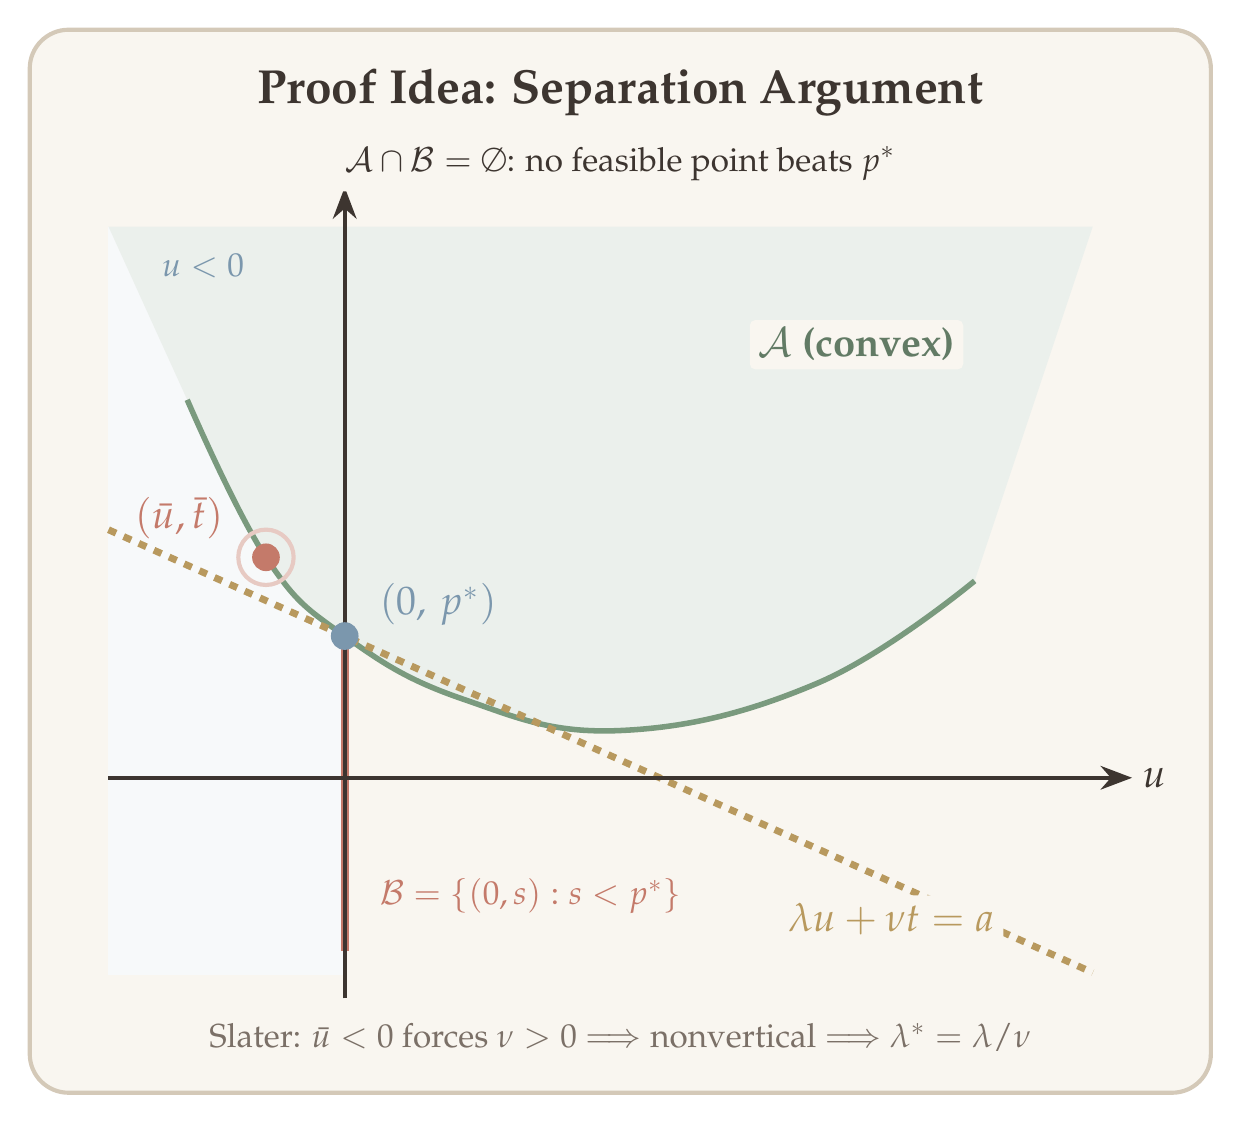
\begin{tikzpicture}[>={Stealth[length=4mm, width=3mm]}, line width=1.5pt]

% Background
\fill[cream, rounded corners=14pt] (-4,-4) rectangle (11,9.5);
\draw[border, line width=1.5pt, rounded corners=14pt] (-4,-4) rectangle (11,9.5);

% Title
\node[font=\LARGE\bfseries, text=dkbrown] at (3.5,8.7)
  {Proof Idea: Separation Argument};

% === Fills drawn BEFORE axes ===

% Light shading for u<0 region
\fill[stblue!6] (-3,-2.5) rectangle (0,7);

% Epigraph set A (convex, extends upward)
\begin{scope}
\clip (-3,-2.5) rectangle (9.5,7);
\fill[sage!15]
  plot[smooth, tension=0.7] coordinates {
    (-2,4.8) (-1,2.8) (0,1.8) (1.5,1.0) (3.5,0.6) (6,1.2) (8,2.5)
  } -- (9.5,7) -- (-3,7) -- cycle;
\draw[sage, line width=2pt]
  plot[smooth, tension=0.7] coordinates {
    (-2,4.8) (-1,2.8) (0,1.8) (1.5,1.0) (3.5,0.6) (6,1.2) (8,2.5)
  };
\end{scope}

% Set B: ray on the t-axis below p* (terracotta)
\draw[terracotta, line width=3pt] (0,-2.2) -- (0,1.8);
\draw[terracotta, line width=1.5pt, fill=cream] (0,1.8) circle (4pt);
\node[font=\large\bfseries, text=terracotta, anchor=west] at (0.3,-1.5)
  {$\mathcal{B} = \{(0,s) : s < p^*\}$};

% Nonvertical separating hyperplane: lambda*u + nu*t = a
% Line passes near (0, p*) with slope -lambda/nu, say slope = -0.45
% t = p* - 0.45*u => at u=-3: t=1.8+1.35=3.15; at u=9: t=1.8-4.05=-2.25
\begin{scope}
\clip (-3.5,-3) rectangle (10,7.5);
\draw[rwgold, line width=2.5pt, dashed]
  (-3, {1.8+0.45*3}) -- (9.5, {1.8-0.45*9.5});
\end{scope}

% === Axes (drawn AFTER fills) ===
\draw[->, dkbrown, line width=1.5pt] (-3,0) -- (10,0)
  node[right, font=\Large, text=dkbrown] {$u$};
\draw[->, dkbrown, line width=1.5pt] (0,-2.8) -- (0,7.5)
  node[above, font=\Large, text=dkbrown] {$t$};

% === Key points and labels ===

% p* on the t-axis
\fill[stblue] (0,1.8) circle (5pt);
\node[font=\Large\bfseries, text=stblue, anchor=west] at (0.3,2.2)
  {$(0,\, p^*)$};

% Slater point in u<0 region, clearly inside A
\fill[terracotta] (-1,2.8) circle (5pt);
\draw[terracotta!40, line width=1.5pt] (-1,2.8) circle (10pt);
\node[font=\Large\bfseries, text=terracotta, anchor=east] at (-1.4,3.3)
  {$(\bar{u}, \bar{t})$};

% Label for A
\node[font=\Large\bfseries, text=sage!80!black,
      fill=cream, inner sep=3pt, rounded corners=2pt] at (6.5,5.5)
  {$\mathcal{A}$ (convex)};

% u<0 label
\node[font=\large, text=stblue] at (-1.8,6.5) {$u < 0$};

% Separating hyperplane label
\node[font=\Large, text=rwgold, fill=cream, inner sep=3pt, rounded corners=2pt,
      anchor=west] at (5.5,-1.8)
  {$\lambda u + \nu t = a$};

% Annotation: A cap B = emptyset
\node[font=\large, text=dkbrown, fill=cream, inner sep=4pt,
      rounded corners=3pt] at (3.5,7.8)
  {$\mathcal{A} \cap \mathcal{B} = \emptyset$: no feasible point beats $p^*$};

% Step annotations along the bottom
\node[font=\large, text=wmgray, align=center] at (3.5,-3.3)
  {Slater: $\bar{u} < 0$ forces $\nu > 0$
   $\Longrightarrow$ nonvertical
   $\Longrightarrow$ $\lambda^* = \lambda/\nu$};

\end{tikzpicture}
\end{document}
